% !TEX root = main.tex
% !TEX encoding = UTF-8
% !TEX program = pdflatex

\section{Results}
    We made several simulations in order to see the behaviour of this three different networks.
    The spread of disease in the two synthetic network is faster than the real network and in addition, the number of people reached is lower in the real network.
    
    For our test we set the parameter $|V|=N=1000$, $\beta = 0.01$ and $\gamma= 0.04$.
    
    The two synthetic network have a strongest connectivity and also if the average degree of this two network is very low, around 20 - 50 link per node Fig.\ref{fig:RandomDegree} and Fig.\ref{fig:PrefAttachDegree}, compared to the other one , around 175 link per node as we can see in the Fig.\ref{fig:FacebookDegree}, the infection is propagated in a easy way.
    This maybe because the Facebook network is structured in 8 cluster and this division characterise the spread of disease, in particular we can see in Fig.\ref{fig:FacebookSIR} the infected line sometime have some evident waves. This is because the spread among different cluster is difficult and need more time.
   
    Another difference is the curve of the infected person, in fact as we can see in the Fig.\ref{fig:FacebookDegree}, Fig.\ref{fig:RandomSIR} and Fig.\ref{fig:PrefAttachSIR} they have different behaviour. The two Synthetic network have a very similar shape, but the random network have a very fast spread, in fact in only 18 days this disease, with the same spread percentage, reached everybody although in the Preferential Attachment network need about 38 days to cover almost everybody and in the real network need about 55 days.
    
    The curve that represents the infected person is strongly related to the number of links and in particular with the network structure. So because in the real world the society is structured in community we should find the best approximation of this in order to make accurate prevision.
    
    So in conclusion the Preferential Attachment network has make able to have a better understand of real world disease spread. Obviously with more adjustments we could reach a better simulation of a real network. This is justified also from the average degree, in fact, the curve of the real network is more close to the curve of preferential attachment network rather than to the random network.
    
    \begin{figure}[t]
        \centering
        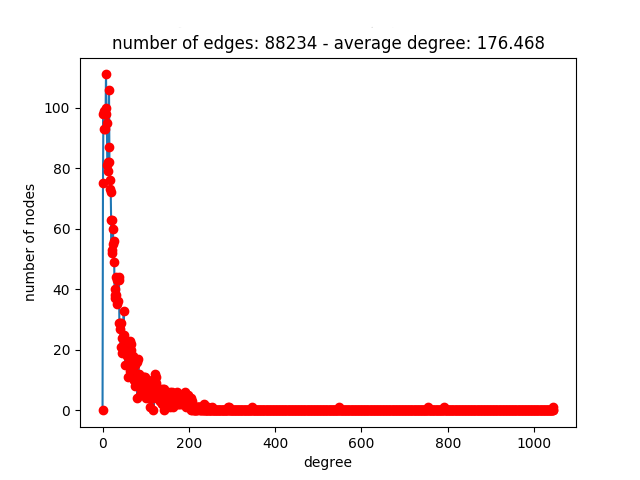
\includegraphics[width=\linewidth]{Figure/Degree_Histogram_Facebook.png}
        \caption{Facebook network degree}
        \label{fig:FacebookDegree}
    \end{figure}
    
    \begin{figure}[t]
        \centering
        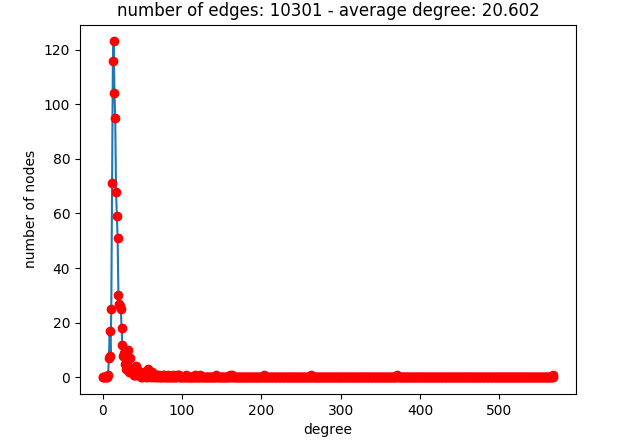
\includegraphics[width=\linewidth]{Figure/Degree_Histogram_PrefAttach.png}
        \caption{Preferential Attachment network degree, N=1000, a = 0.25, m = 4.5}
        \label{fig:PrefAttachDegree}
    \end{figure}
    
    \begin{figure}[t]
        \centering
        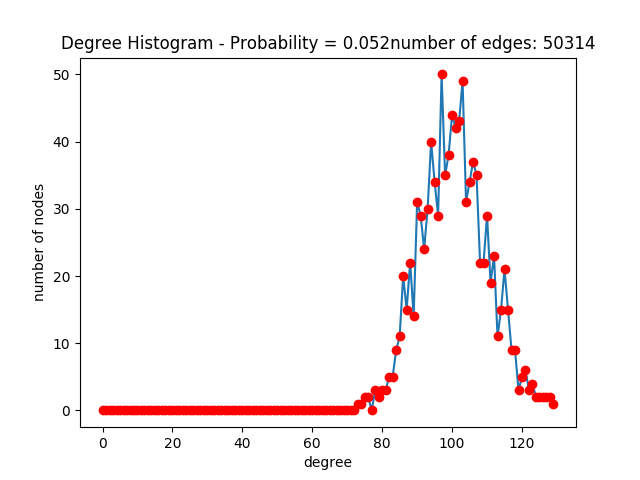
\includegraphics[width=\linewidth]{Figure/Degree_Histogram_Random.png}
        \caption{Random network degree}
        \label{fig:RandomDegree}
    \end{figure}
    
    \begin{figure}[t]
        \centering
        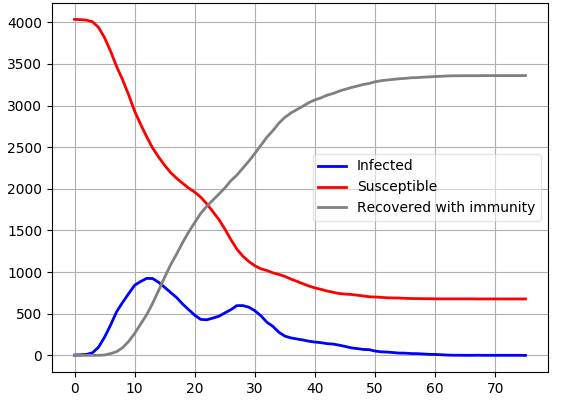
\includegraphics[width=\linewidth]{Figure/SIR_graph_Facebook.png}
        \caption{SIR graph related to Facebook network}
        \label{fig:FacebookSIR}
    \end{figure}
    
    \begin{figure}[t]
        \centering
        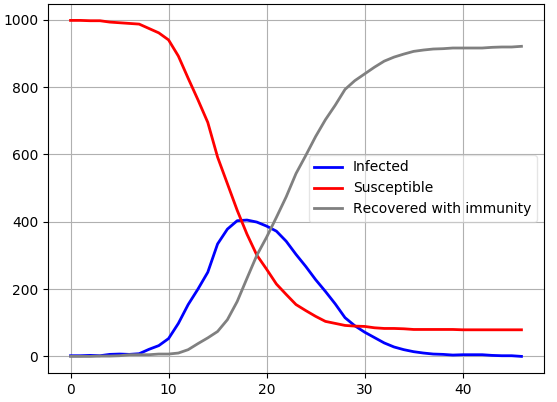
\includegraphics[width=\linewidth]{Figure/SIR_graph_PrefAttach.png}
        \caption{SIR graph related to Preferential Attachment network}
        \label{fig:PrefAttachSIR}
    \end{figure}
    
    \begin{figure}[t]
        \centering
        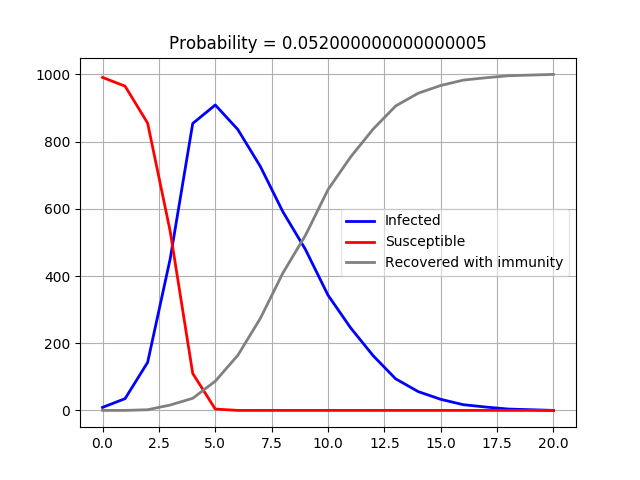
\includegraphics[width=\linewidth]{Figure/SIR_graph_Random.png}
        \caption{SIR graph related to Random network}
        \label{fig:RandomSIR}
    \end{figure}